    %
    { \footnotesize
    \begin{figure}
    \centering
    %
    \begin{subfigure}{.3\textwidth}
        $
        \begin{array}{l}
            N < m < n\\
            \kw{threeNestedWhile}(n, m, N) \triangleq \\
            \clabel{ \assign{i}{0} }^{0} ; \\
                L_1: \ewhile ~ \clabel{i < n}^{1} ~ \edo ~ \\
                \qquad \Big(
                 \highlight{\clabel{\assign{j}{0}}^{2}} ;\\
                 L_3:  \qquad \ewhile ~ \clabel{j < m}^{3} ~ \edo ~ \\
                 \qquad \qquad \Big(
                  \clabel{\assign{j}{j+1}}^{4};
                  \highlight{\clabel{\assign{w}{i}}^{5}};\\
                  L_6:  \qquad \qquad \ewhile ~ \clabel{w < N}^{6} ~ \edo ~
                  \Big(
                    \clabel{\assign{w}{w + 1}}^{7}
                      \Big); \\
                      \qquad \qquad \clabel{\assign{i}{w}}^{8}
                      \Big); \\
                      \qquad \clabel{\assign{i}{i+1}}^{9}
                  \Big)
            \end{array}
            $
    \caption{}
        \end{subfigure}
    \begin{subfigure}{.4\textwidth}
        \begin{centering}
            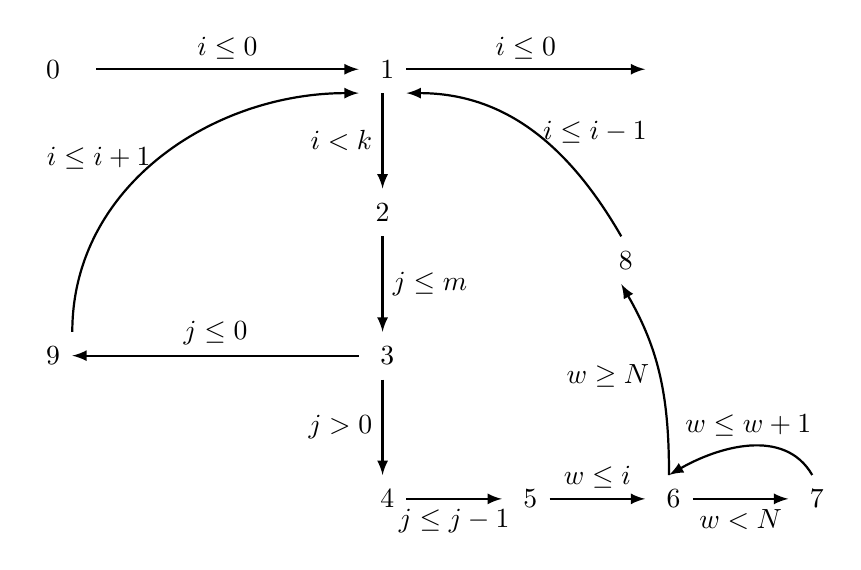
\begin{tikzpicture}[scale=\textwidth/20cm,samples=200]
                \draw[] (-7, 10) circle (0pt) node{{ $0$}};
                \draw[] (0, 10) circle (0pt) node{{ $1$}};
                \draw[] (6, 10) circle (0pt) node {{$\lex$}};
                \draw[] (0, 7) circle (0pt) node{{$2$}};
                \draw[] (0, 4) circle (0pt) node{{ $3$}};
                \draw[] (-7, 4) circle (0pt) node{{ $9$}};
                \draw[] (0, 1) circle (0pt) node{{ $4$}};
                \draw[] (3, 1) circle (0pt) node{{ $5$}};
                \draw[] (6, 1) circle (0pt) node{{ $6$}};
                \draw[] (9, 1) circle (0pt) node{{ $7$}};
                \draw[] (5, 6) circle (0pt) node{{ $8$}};
                % Counter Variables
                %
                % Control Flow Edges:
                \draw[ thick, -latex] (-6, 10)  -- node [above] {$i \leq 0$}(-0.5, 10);
                \draw[ thick, -latex] (0, 9.5)  -- node [left] {$i < k$} (0, 7.5) ;
                \draw[ thick, -latex] (0, 6.5)  -- node [right] {$j \leq m$} (0, 4.5) ;
                \draw[ thick, -latex] (0, 3.5)  -- node [left] {$j > 0$} (0, 1.5) ;
                \draw[ thick, -latex] (-0.5, 4)  -- node [above] {$j \leq 0$} (-6.5, 4) ;
                \draw[ thick, -latex] (-6.5, 4.5)  to  [out=90,in=180]  node [left] {$i \leq i + 1$ }(-0.5, 9.5);
                \draw[ thick, -latex] (0.5, 10)  -- node [above] {$i \leq 0$}  (5.5, 10);
                \draw[ thick, -latex] (0.5, 1)  -- node [below] {$j \leq j - 1$}  (2.5, 1);
                \draw[ thick, -latex] (3.5, 1)  -- node [above] {$w \leq i$}  (5.5, 1);
                \draw[ thick, -latex] (6.5, 1)  -- node [below] {$w < N$}  (8.5, 1);
                \draw[ thick, -latex] (6, 1.5)  to [out=90,in=-60] node [left] {$w \geq N$}  (5, 5.5);
                \draw[ thick, -latex] (9, 1.5)  to  [out=120,in=30] node [above] {$w \leq w + 1$}  (6, 1.5);
                \draw[ thick, -latex] (5, 6.5)  to  [out=120,in=0]  node [right] {$i \leq i - 1$ }(0.5, 9.5);
                \end{tikzpicture}
    \caption{}
    \end{centering}
    \end{subfigure}
\begin{subfigure}{.2\textwidth}    
\begin{centering}
    $
    \begin{array}{l}
        \tpath_0 = (0 \to 1)
        \\
        \tpath_1 = (1 \to 2 \to 3)
        \\        
        \tpath_2 = (3 \to 4 \to 5 \to 6)
        \\
        \tpath_3 = (6 \to 7 \to 6)
        \\
        \tpath_6 = (1 \to \lex)
        \\
        \tpath_4 = (6 \to 8 \to 3)
        \\
        \tpath_5 = (3 \to 9 \to 1)
    \end{array}
$
\caption{}
\end{centering}
\end{subfigure}
    \caption{
    (a) An example of three nested loops with related iterator variables.
    (b) The Abstract Transition Graph for $\kw{threeNestedWhile}(n, m, N)$.}
        \label{fig:threeWhile}
    \end{figure}
    }